\section{Architecture}
\label{sec:architecture}
% ANTONELLA
The system created allows the user to enter a question in natural language, this question the system intends to translate it into a formal query through the ontology-based grammar-based language analysis and to which ontology answers in Based on the content of the application.
\begin{itemize}
	\item Grammar generation
	\item Linguistic analysis of demand and answer to the user
\end{itemize}

\subsection{Grammar generator}
Grammar has been assumed made up of two parts: one depending on ontology, and another independent. The domain specific grammar refers to the part that contains the lexical entries like individuals, concepts and properties contained in the ontology. The ontological independent part contains expressions like auxiliary verbs, determiners, wh-words, and so on.

Generally what he does is represented as follows:

\begin{figure}[H]
   \centering
    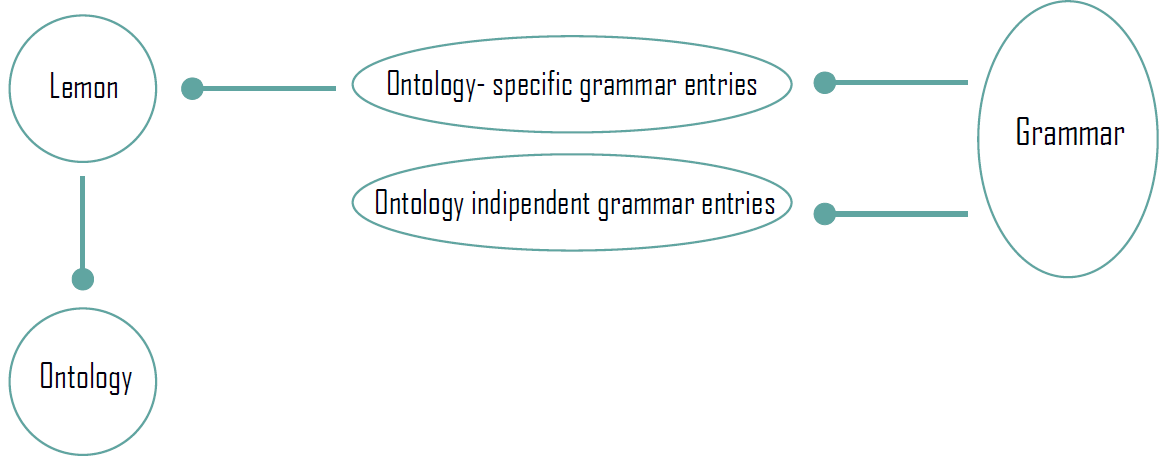
\includegraphics[scale=0.5]{./fig/grammar}
    \label{fig:grammar}
    \caption{The Grammar.}
\end{figure}

Both parts of the grammar use the main linguistic representations or each grammar is represented as a pair of syntactic and semantic representations. As a syntactic representation, Lexicalized Tree Adjoining Grammar (LTAG) is used. As semantic representations we take Dudes.

The first step in generating a grammar from a given ontology is to enrich the ontology with information about its verbalization. To achieve this we leverage LexInfo, which uses a general frame to create a declarative specification of the lexicon-ontology interface by connecting concepts of the ontology to information about their linguistic realization, i.e. word forms, morphology, sub-categorization frames and how syntactic and semantic arguments correspond to each other. The lexical entries specified by LexInfo are then used to generate grammar entries, i.e. indexed LTAG/DUDES.

\subsection{Ontoqa}
The system provides the user with an intuitive interface to submit questions, expressed in English natural language.

The natural language question is processed by the parser to generate the corresponding LTAG/DUDES representation, from which a formal SPARQL query can be obtained.
%After the disambiguation and obtaining of the SLTAG of our universe of speech, we generate a formal query. The formal query will be submitted to the ontology that will return us an answer. 
Finally, the query is submitted to the ontology, thus retrieving the output answer.
The procedure is shown in the Figure.

%The system allows a user to submit, via an intuitive interface, a natural-language question in English.

%Given the question in Natural Language, a parsing is applied that constructs an LTAG derivative tree considering only the syntactic part of the grammatical voices involved.

%Subsequently, syntactic and semantic composition rules apply to the construction of a tree in accordance with the LTAG derivation tree and DUDES semantics.

%In general, what happens is that LTAG provides substitution and adjunction rules while DUDES semantics provides rules as saturation operations that are interpreted as substitutions and a union operation that interprets the adjoin.



\begin{figure}[H]
   \centering
    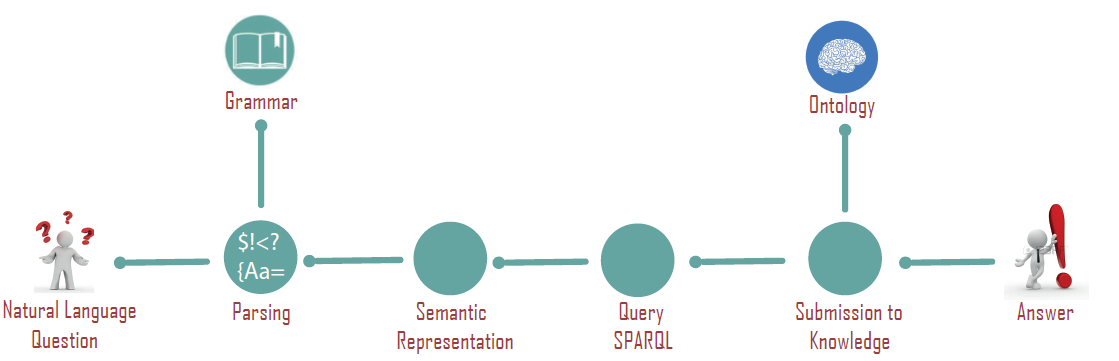
\includegraphics[scale=0.5]{./fig/ontoqa}
    \label{fig:ontoqa}
    \caption{The workflow.}
\end{figure}